\section{Simulation Results}
\label{sec:result}





A 256-subcarrier \gls{siso} \gls{ofdm} system is considered. Bob and Eve channels are assumed to be uncorrelated. Each subcarrier is Rayleigh distributed and there is no correlation between subcarriers. As a reminder, the overall channel energies are normalized to unity for each channel realization. Bob's \gls{csi} is assumed to be perfectly known at Alice. Bob and Eve have the same level of noise. Simulations with 100 channel realizations and 300 \gls{ofdm} blocks were performed using a 4-QAM modulation scheme. 


\subsection{Decoding results}
\textit{The presented results in this section were obtained for the scenario where Eve has the same capabilities as Bob. This is subject to further completion where the different decoding structures will be included.}
\begin{figure}[htb!]
    \centering
    \centerline{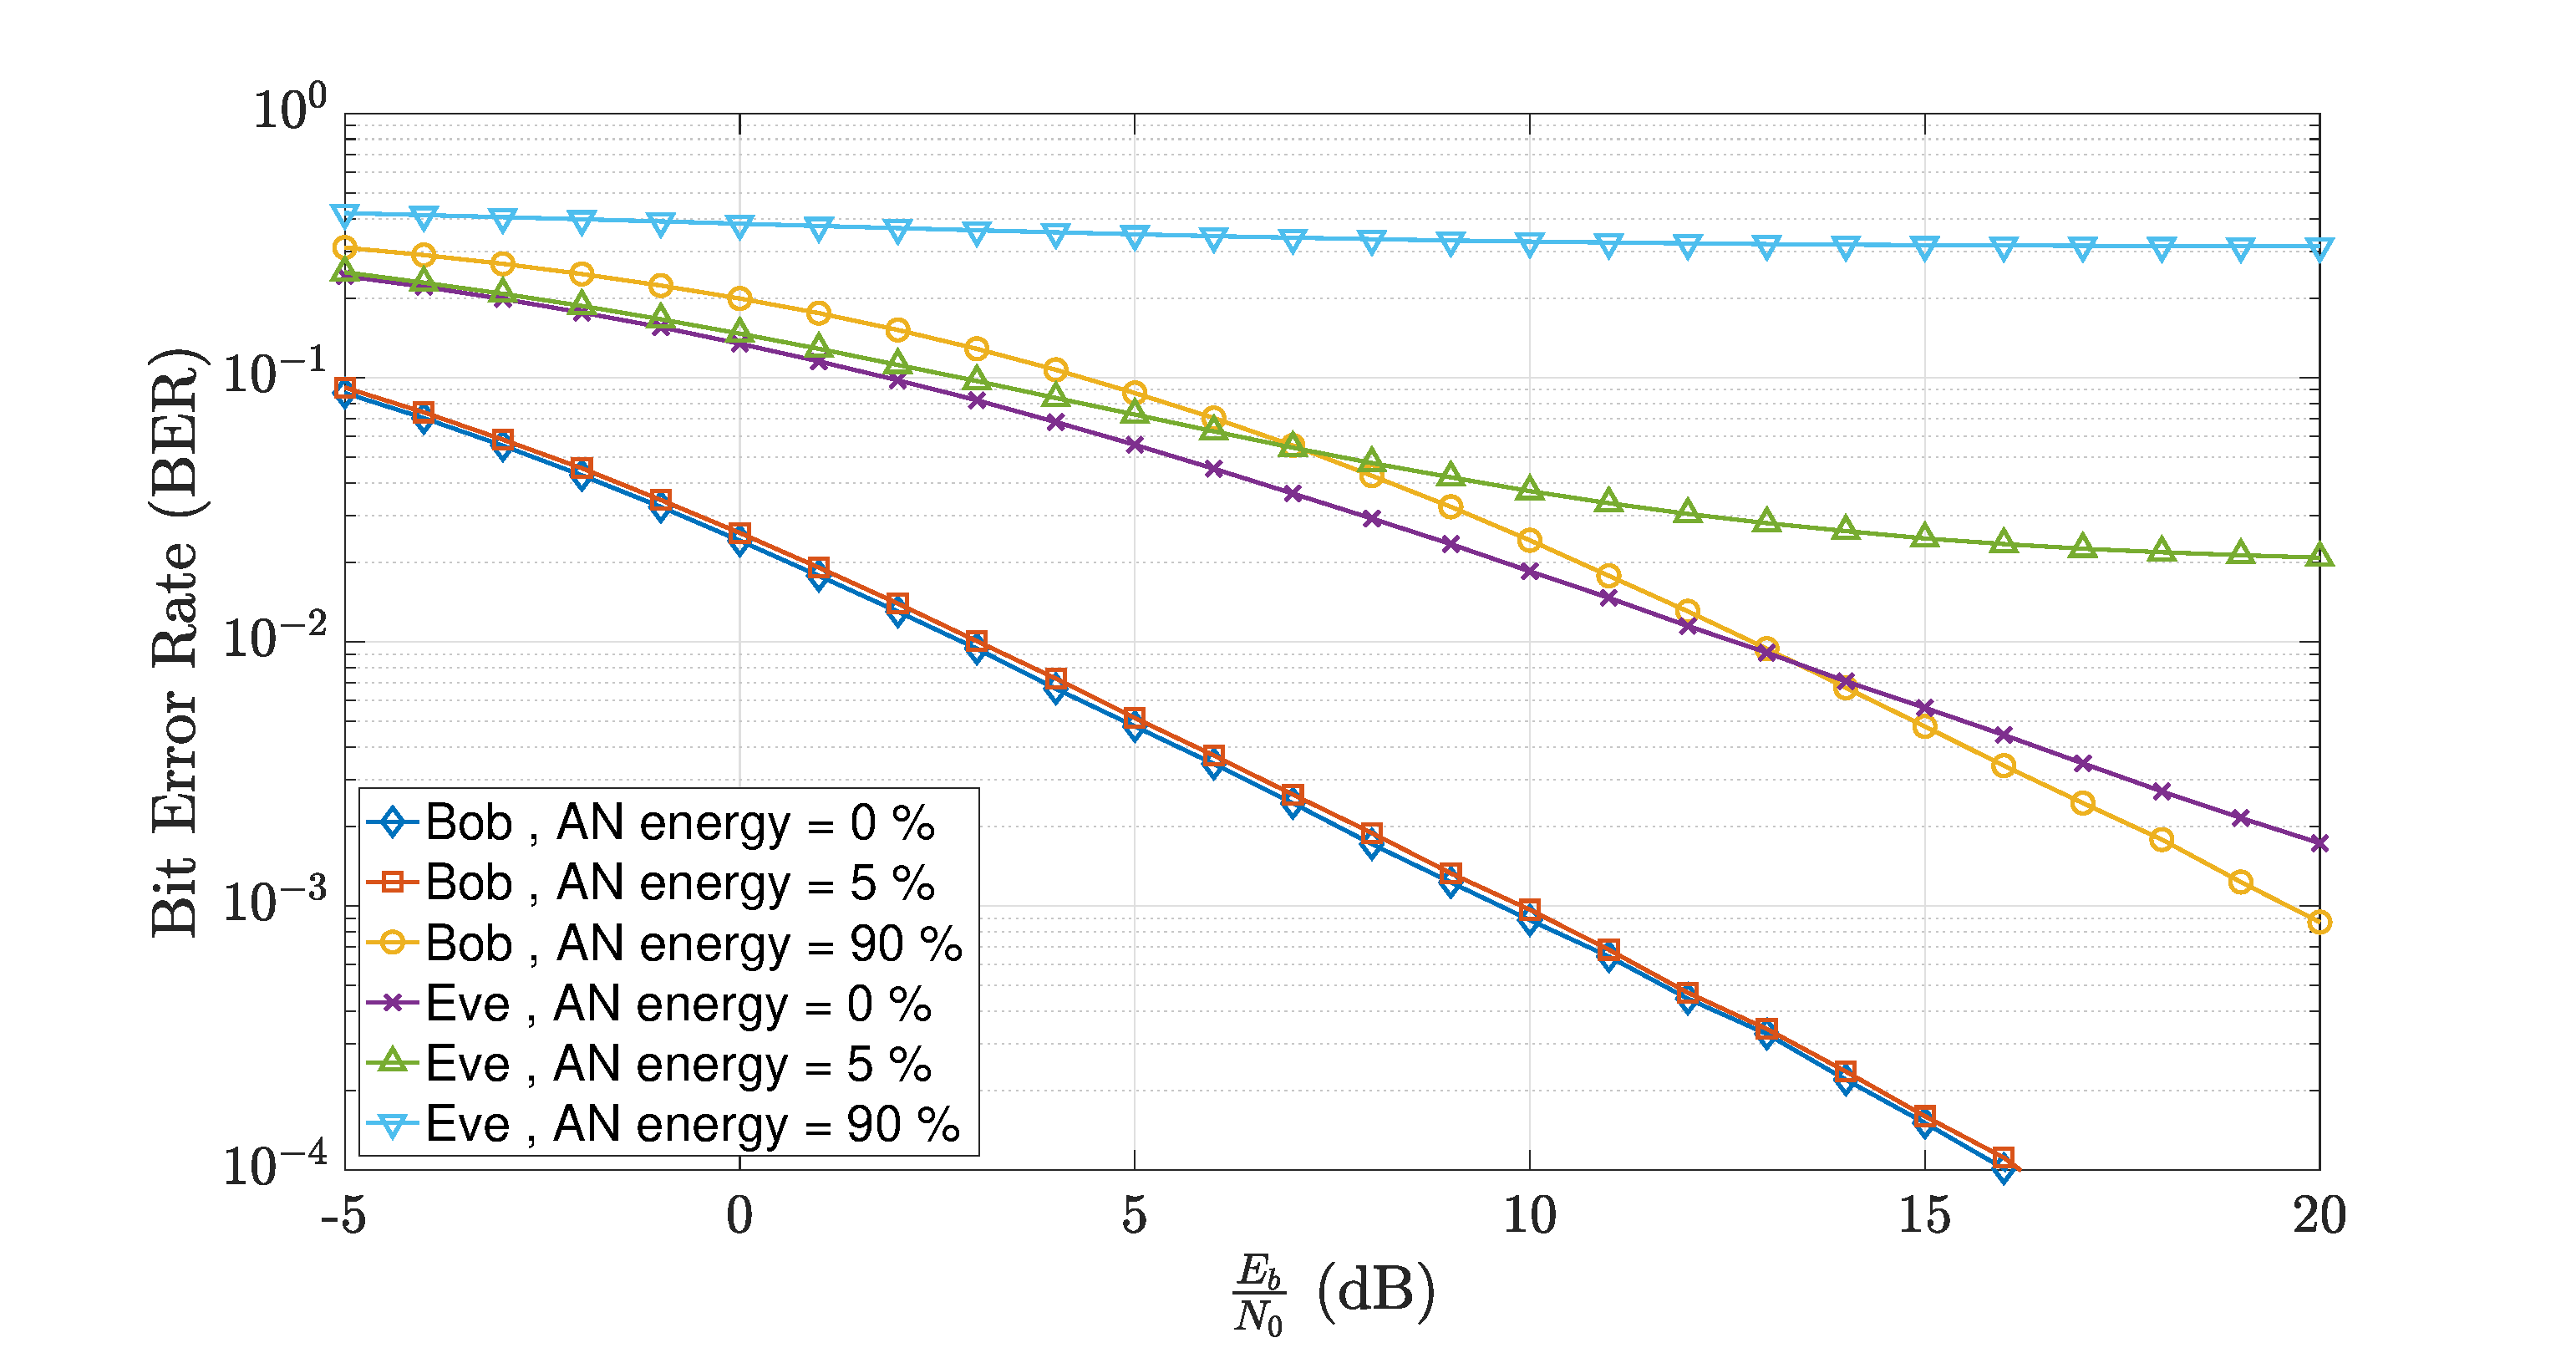
\includegraphics[width = .65\textwidth]{graphs/ber_ebno_alpha_bor_globcom.eps}}
    \caption{BER as a function of the level of noise for different AN energy values, \gls{bor} = 4}
    \label{fig:ber_ebno}
\end{figure}

\begin{figure}[htb!]
    \centering
    \centerline{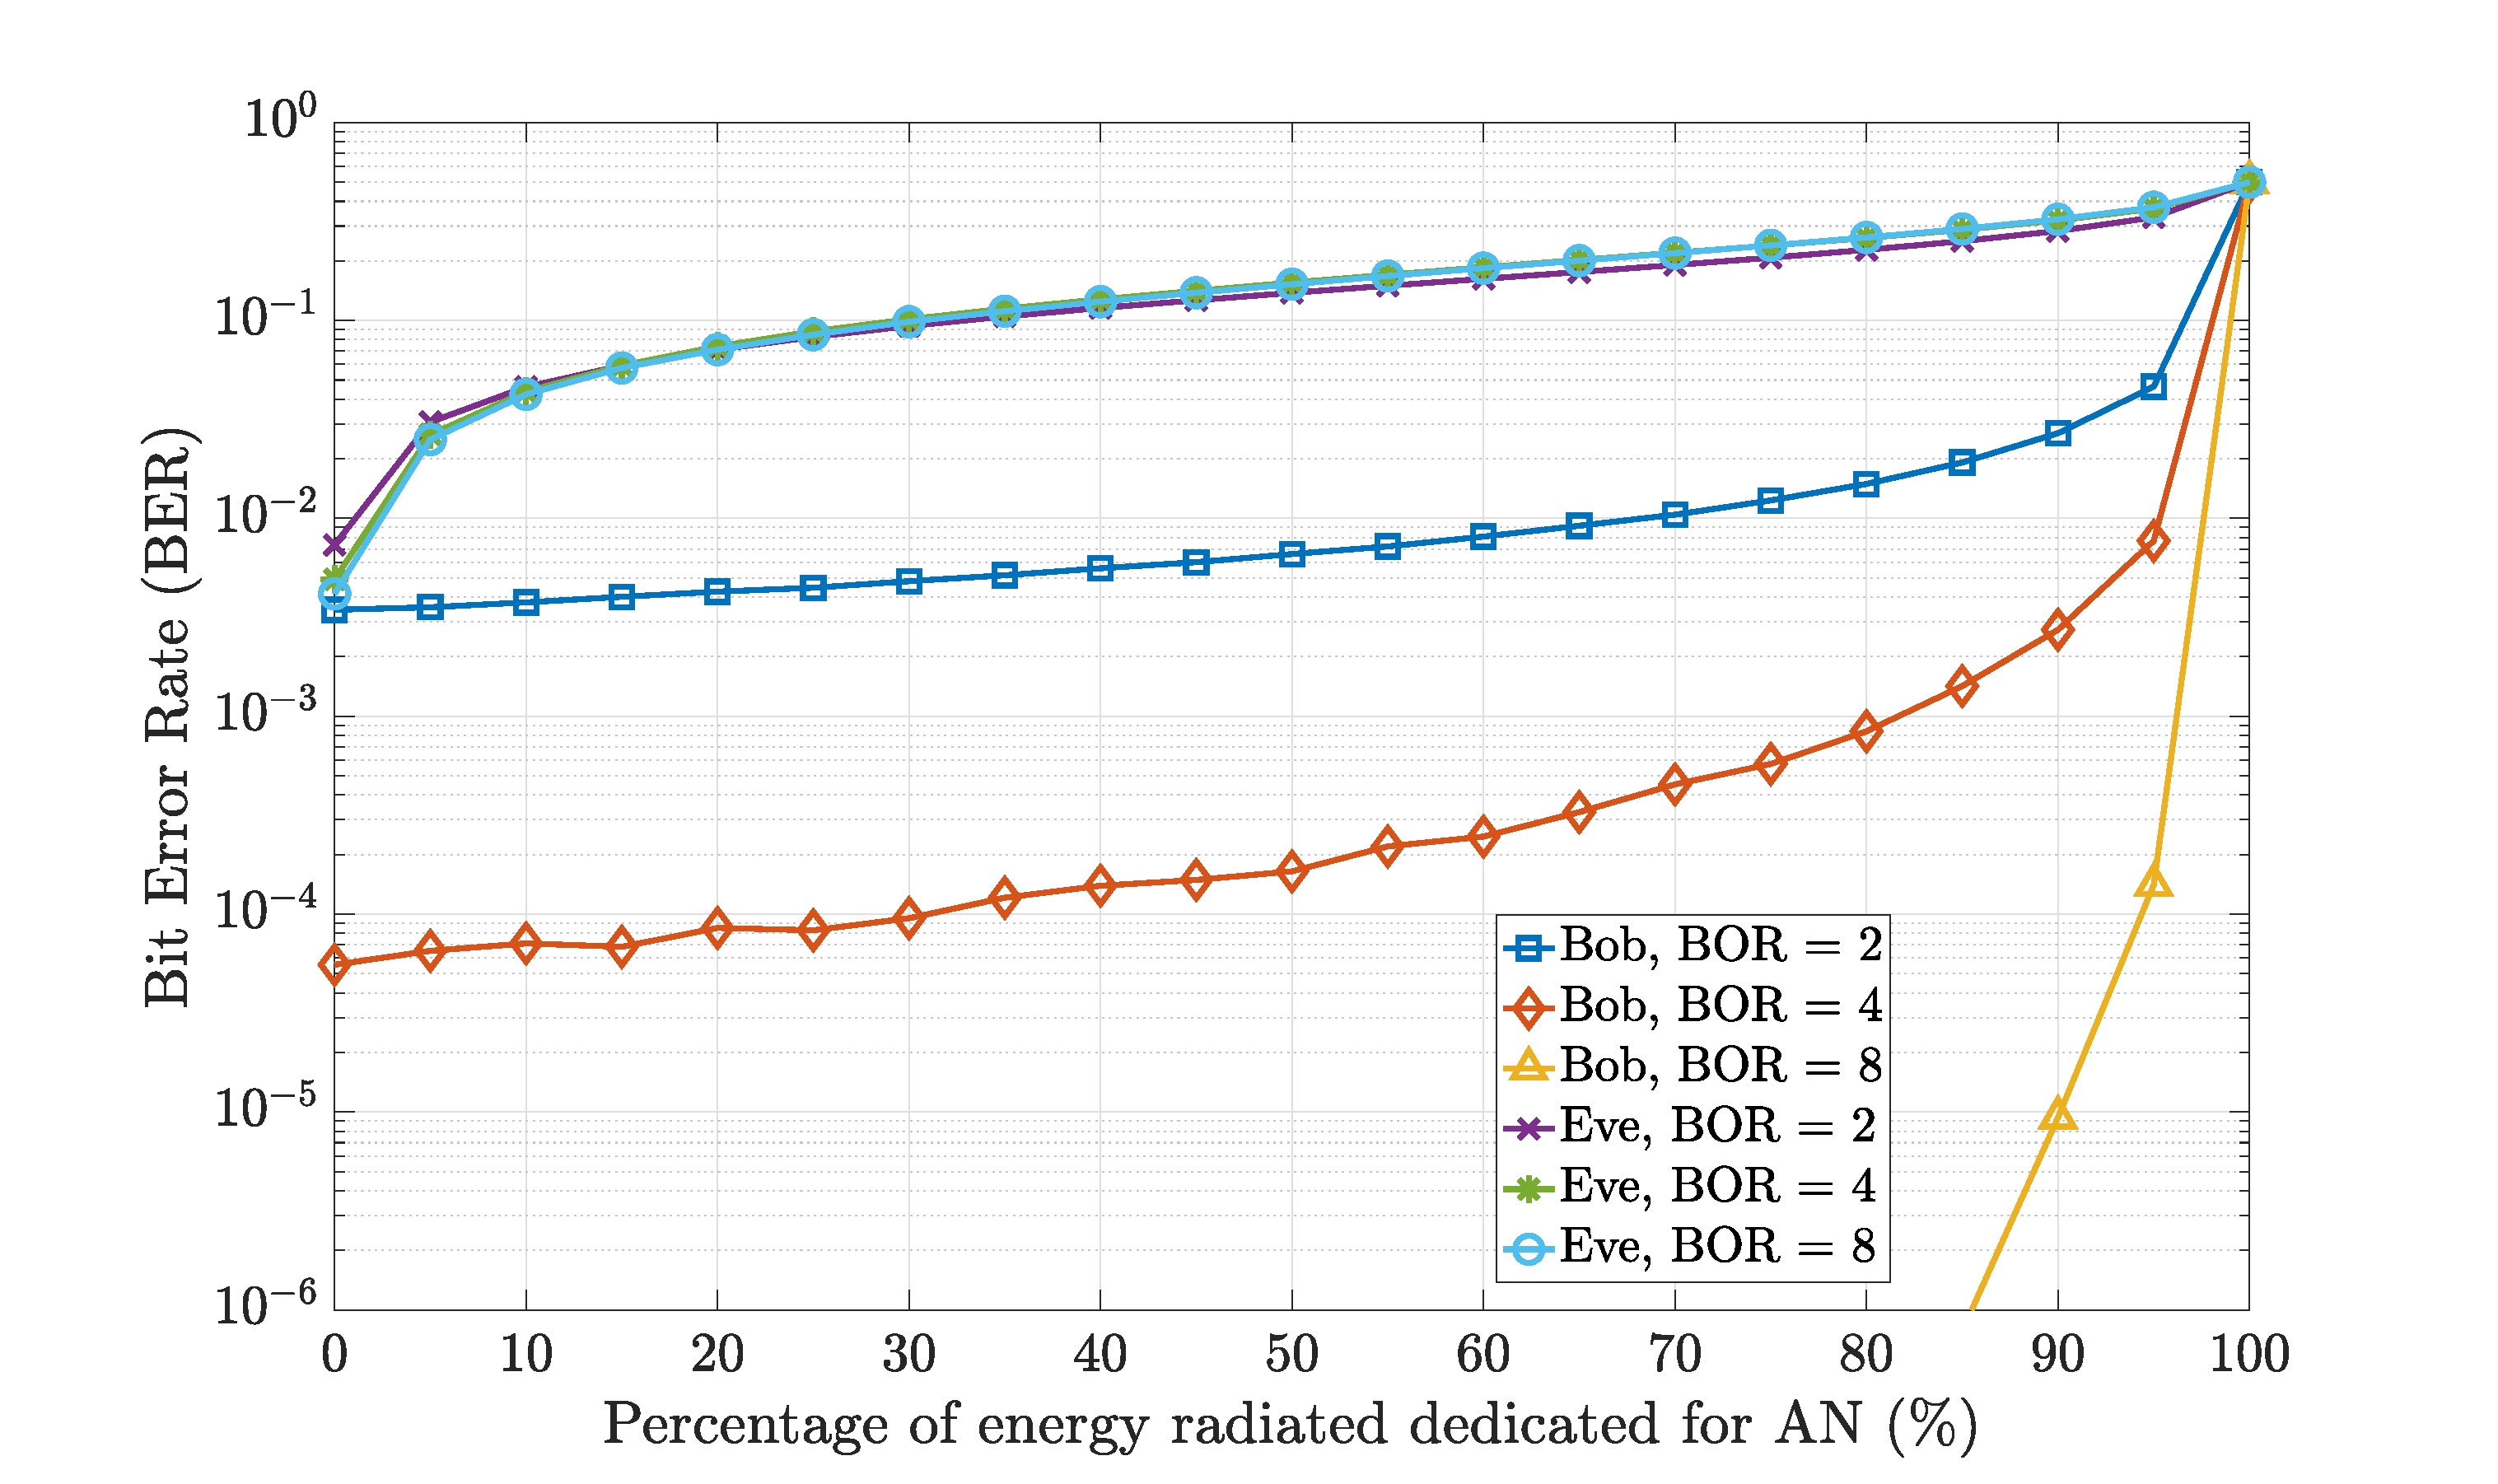
\includegraphics[width = .65\textwidth]{graphs/ber_alpha_bor_ebno_globcom.eps}}
    \caption{BER as a function of AN energy for different BOR values, $E_b/N_0 = 15$dB}
    \label{fig:ber_alpha}
\end{figure}
Fig. \ref{fig:ber_ebno} and \ref{fig:ber_alpha} show the system performance in terms of \gls{ber} obtained after \gls{zf} equalization at Bob and Eve. In Fig. \ref{fig:ber_ebno}, the \gls{ber} is plotted as a function of $E_b/N_0$, where $E_b$ is the energy per bit, calculated after spreading, and $N_0$ is the noise power spectral density.  Different levels of \gls{an} energy are investigated at fixed \gls{bor}. It can be observed that, as soon as a small amount of radiated energy is dedicated to \gls{an}, e.g., $5\%$, Eve's \gls{ber} strongly increases. At the intended position, the \gls{ber} also increases but much slower. The reason is that the higher the percentage of energy dedicated to \gls{an}, the lower the received useful signal power at Bob. In Fig. \ref{fig:ber_alpha}, the \gls{ber} is plotted as a function of the \gls{an} energy, at fixed $E_b/N_0=15$ dB and different \gls{bor} values. At the unintended position, the \gls{ber} naturally increases with the amount of injected \gls{an}, whatever the \gls{bor} value. At Bob, low \gls{ber} values can be maintained for high \gls{an} power by increasing the \gls{bor}. One can notice that, when $\alpha \to 0$, the \gls{ber} curves all converge to $0.5$, as expected.






\subsection{Secrecy results}
\label{subsec:sec_result}
\subsubsection{Eve and Bob with identical capacities}
\label{subsubsec:sec_result_despreading}
\begin{figure}[ht!]
    \centering
    \centerline{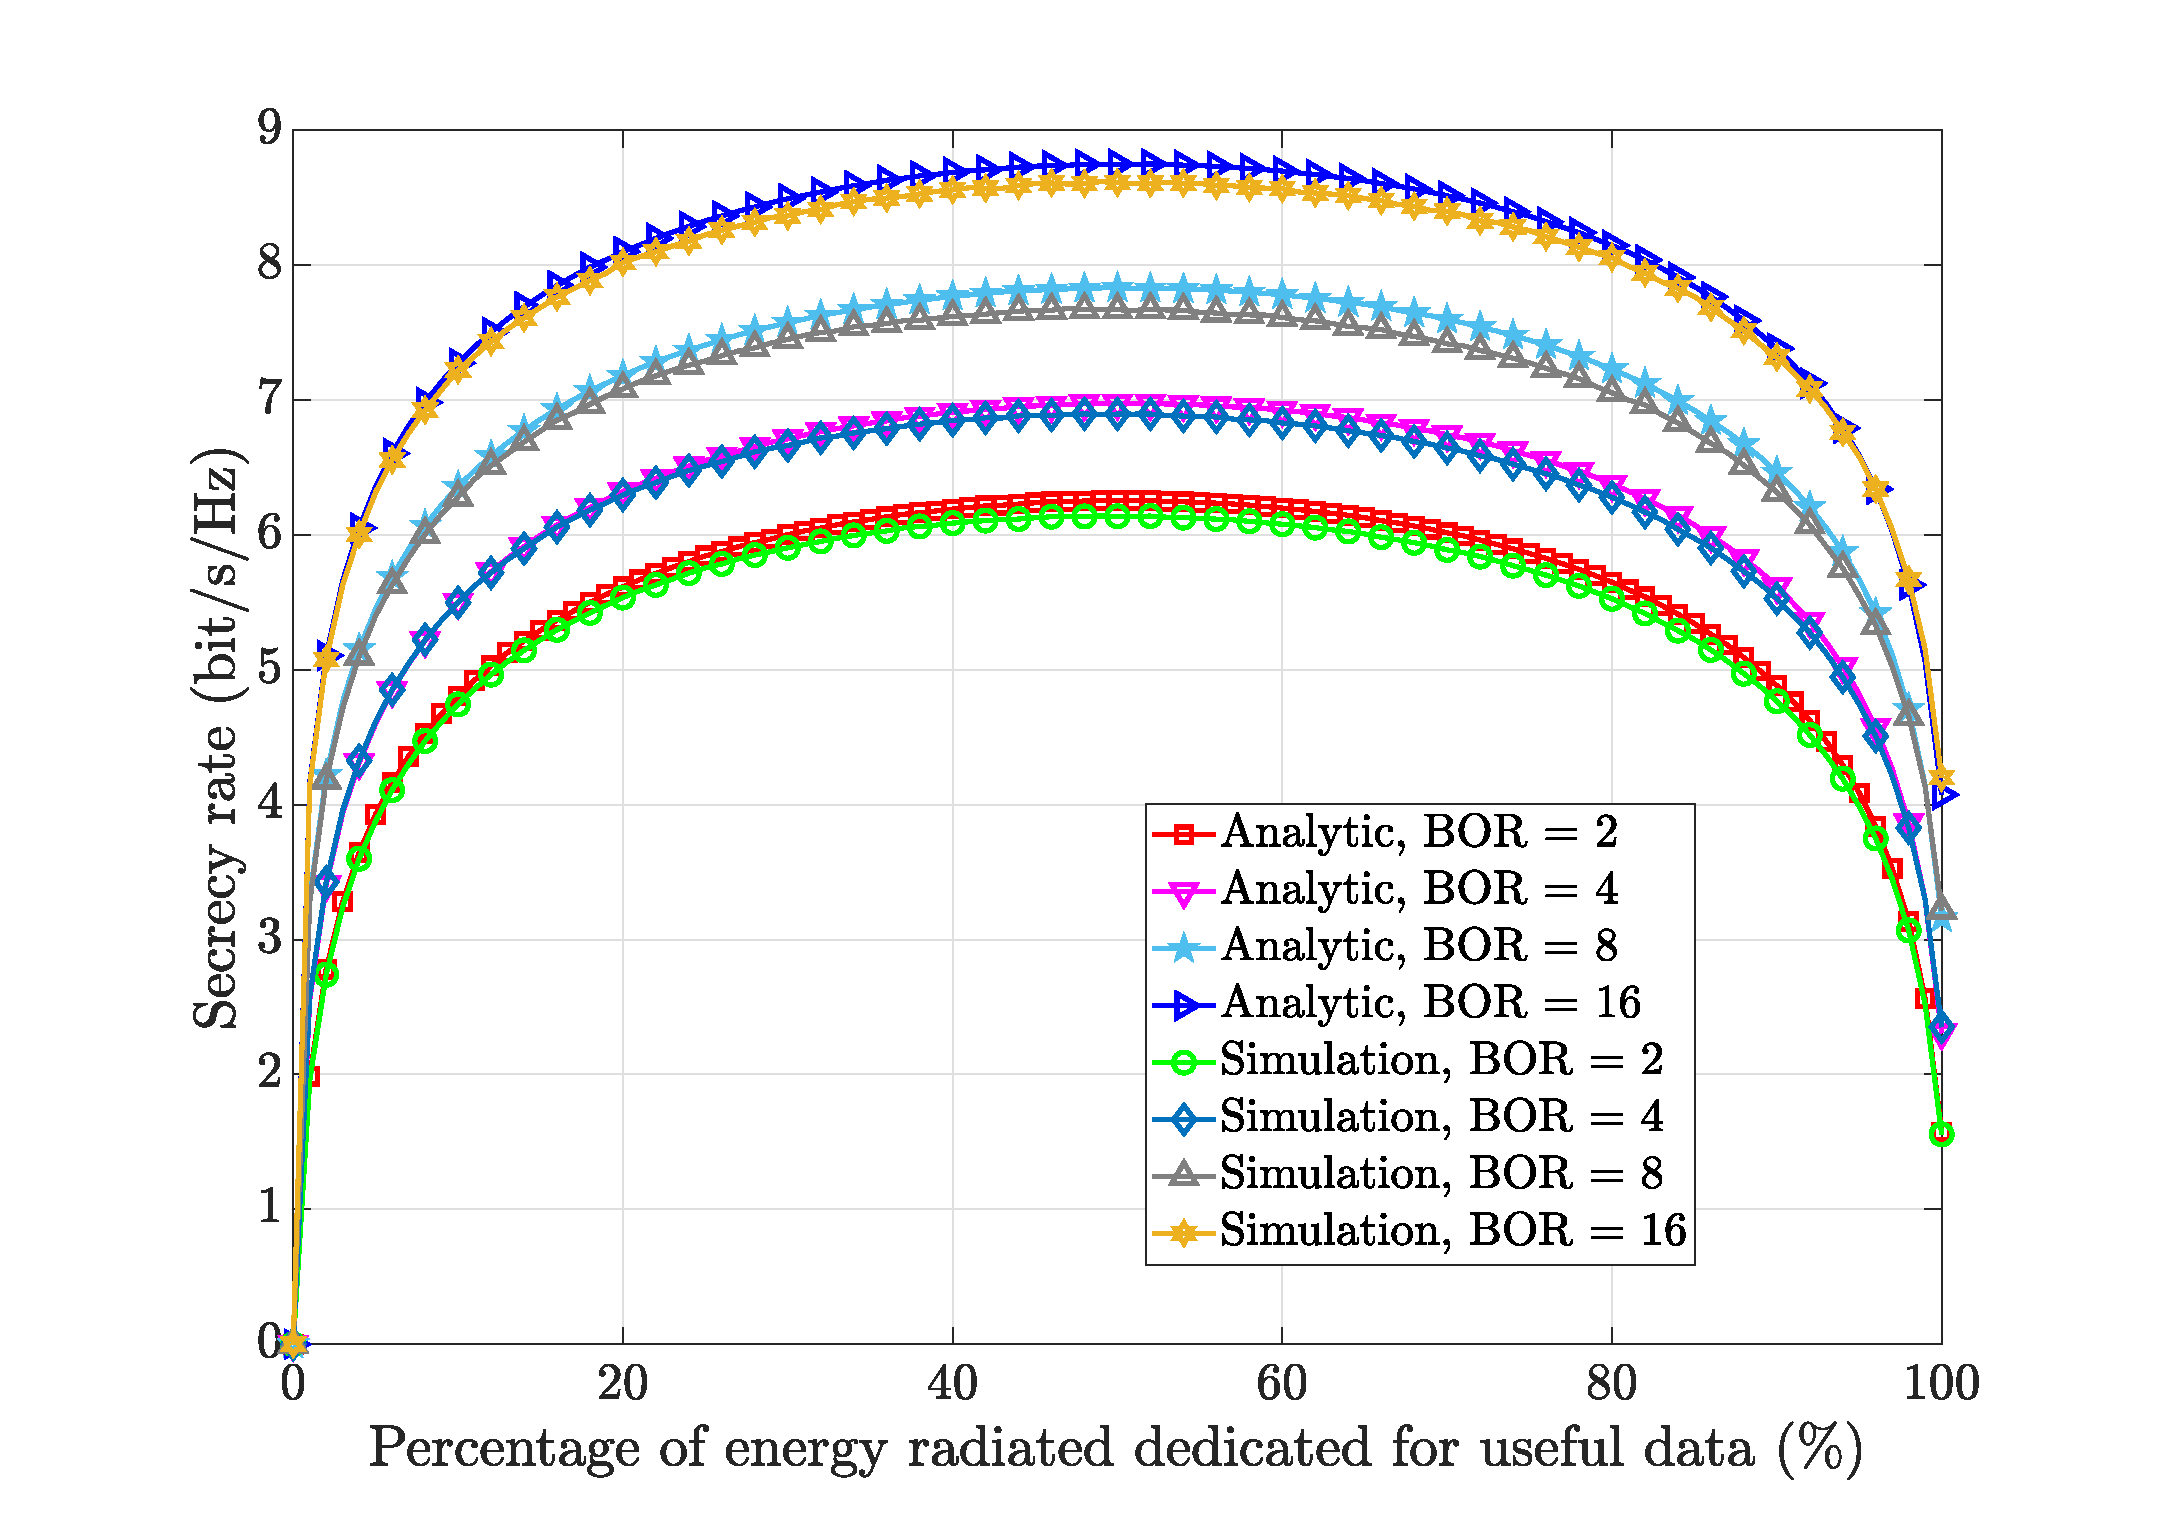
\includegraphics[width = .65\textwidth]{graphs/SR_simu_anal_filt0.eps}}
    \caption{Secrecy Rate curves, analytic vs simulation, Bob and Eve with same capabilities, $E_b/N_0=20$ dB }
    \label{fig:secrecy_alpha_bor}
\end{figure}
\begin{figure}[ht!]
    \centering
    \centerline{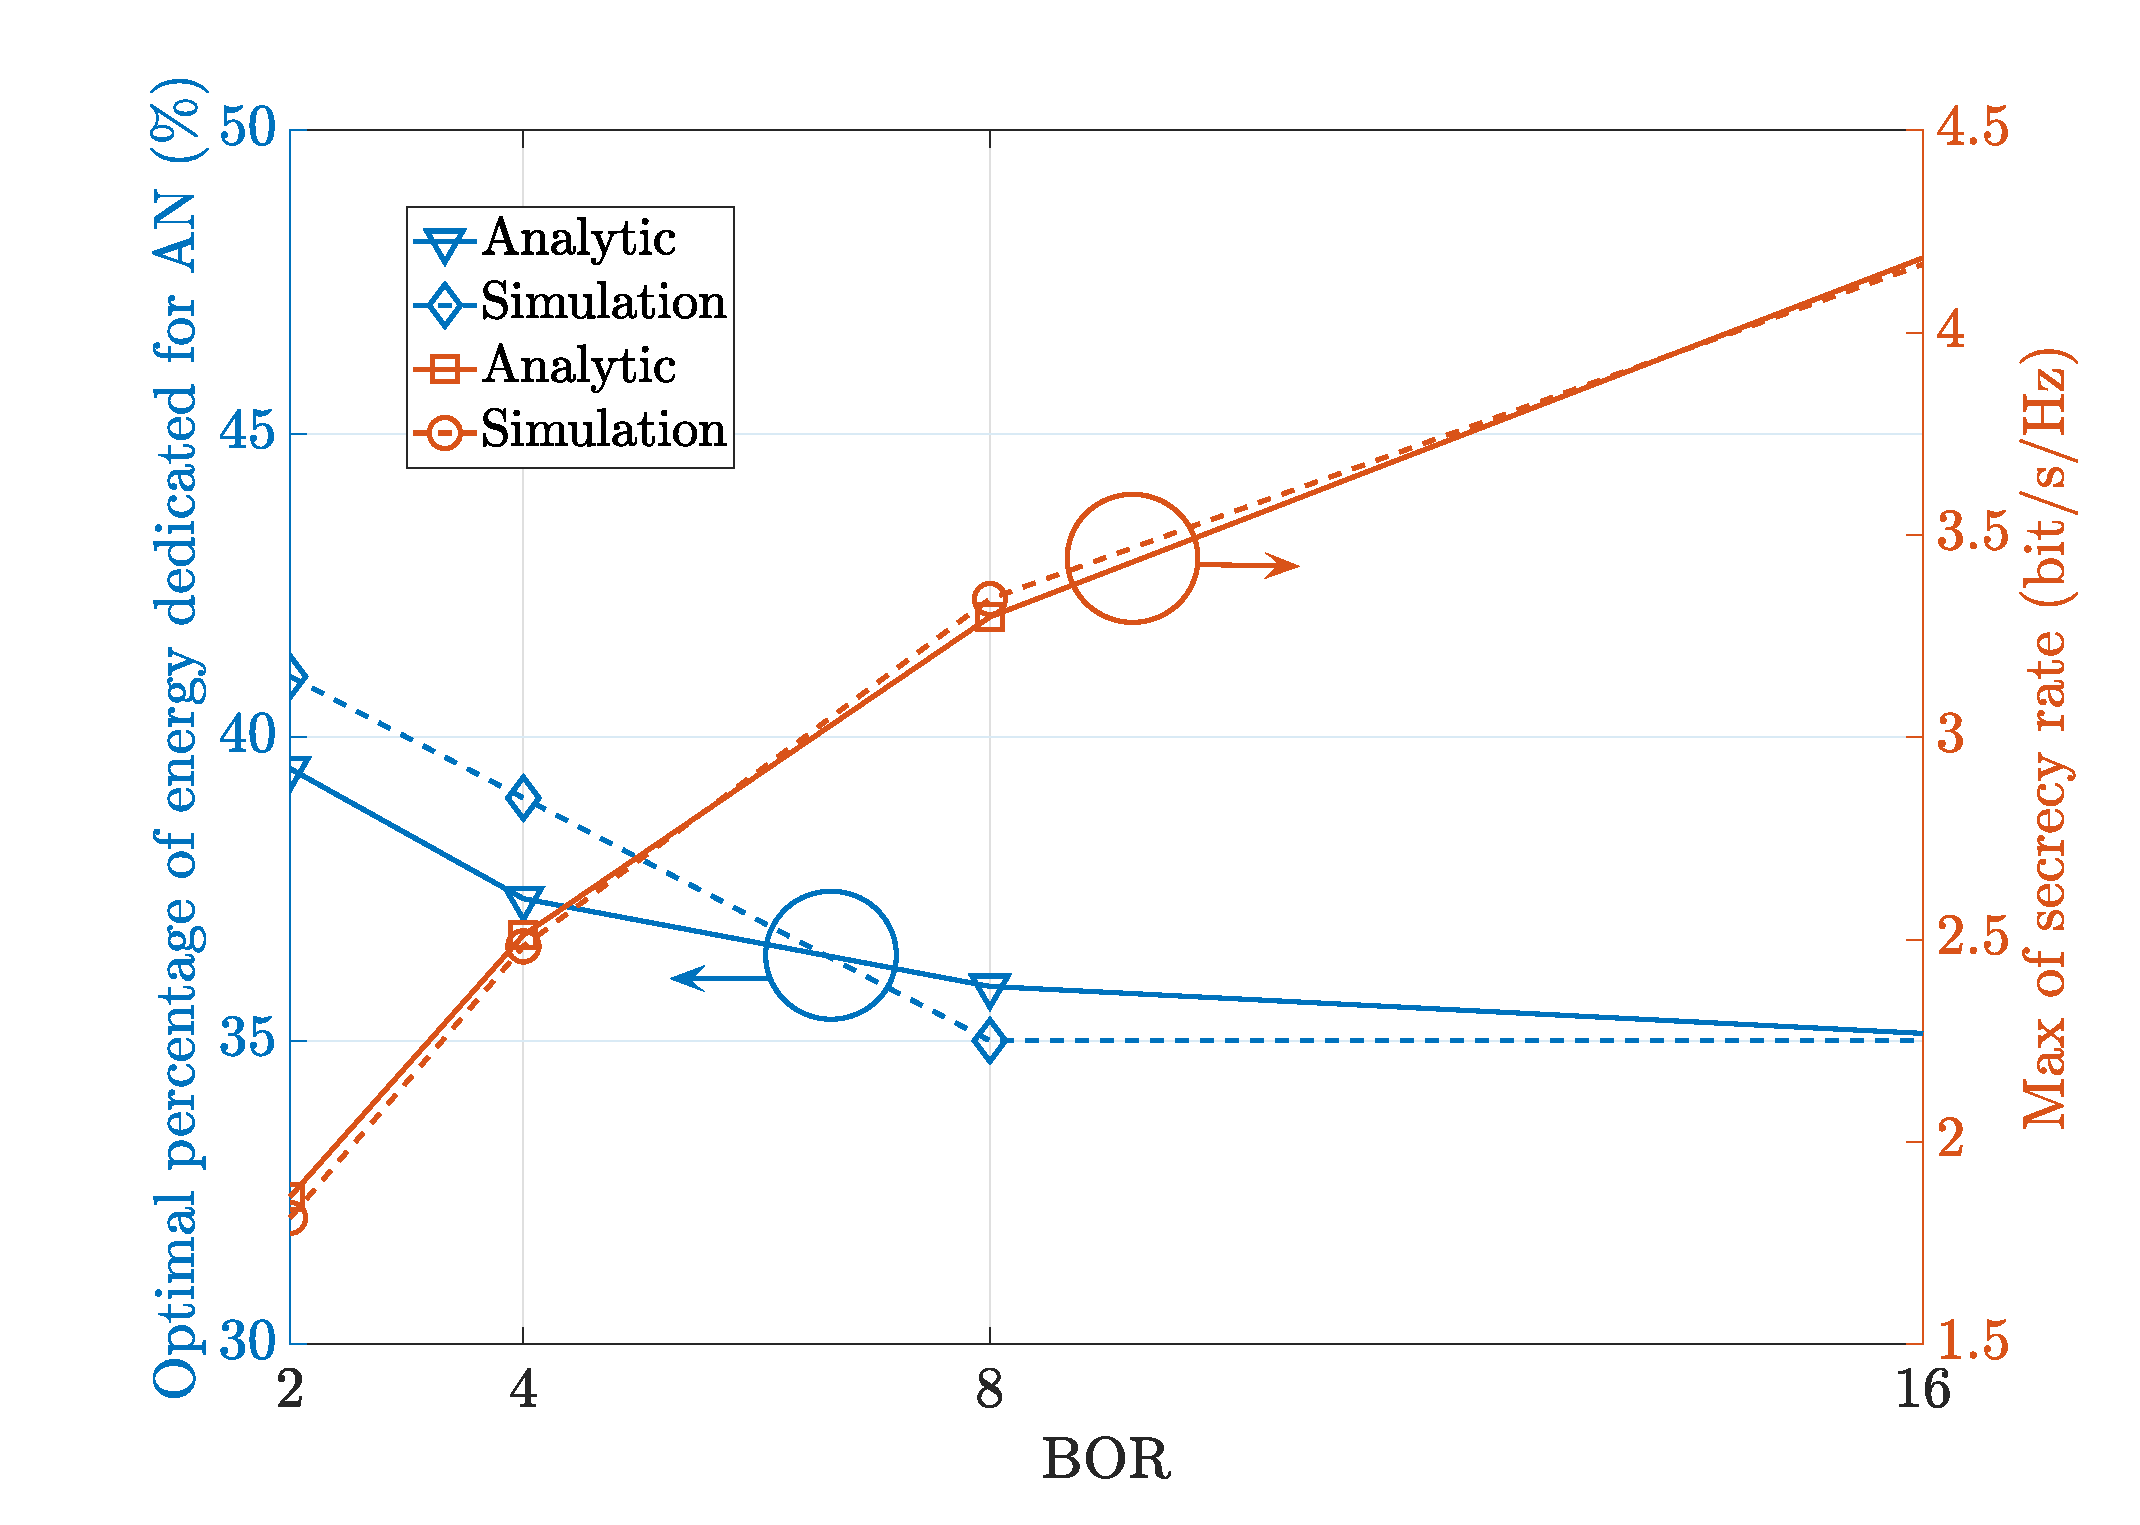
\includegraphics[width = .65\textwidth]{graphs/SR_max.eps}}
    \caption{Optimal amount of AN to inject, Bob and Eve with same capabilities, $E_b/N_0=5$ dB }
    \label{fig:secrecy_alpha_bor_optimal}
\end{figure}
Fig. \ref{fig:secrecy_alpha_bor} shows the \gls{sr} evolution as a function of $\alpha$ for different \gls{bor} values. It is considered that Eve's receiver is equivalent to Bob's one. First, it can be seen that analytic curves, given by (\ref{eq:SR_anal2}), approximate well the simulation curves and remains a tight upper bound for all scenarios.  In addition, the \gls{sr} obtained with the classical \gls{fd} \gls{tr} \gls{siso} \gls{ofdm} system, i.e., no \gls{an} signal, is enhanced with the addition of \gls{an} except for very high percentages of \gls{an}. Furthermore, the \gls{sr} increases when the \gls{bor} becomes higher because the \gls{tr} gain becomes larger at Bob for higher \gls{bor} values but not at Eve. No more secrecy is obtained when $\alpha \to 0$, since the \gls{sinr}'s at Bob and Eve drop to zero.\\
Fig. \ref{fig:secrecy_alpha_bor_optimal} illustrates the values of $\alpha_{opt}$ given by (\ref{eq:best_alpha}) that maximize the \gls{sr} determined from the closed-form approximation (\ref{eq:SR_anal2}), as well as obtained from the numerical simulations. The analytic estimation of the optimal amount of \gls{an} energy is not perfect but, the resulting simulated \gls{sr} is very close to the maximal \gls{sr}. The reason can be observed in Fig. \ref{fig:secrecy_alpha_bor} where the \gls{sr} varies very slowly about its maximum when $\alpha$ changes. So, for a given \gls{bor} value, Alice can make a rough determination of $\alpha_{opt}$ and therefore the available \gls{sr}, if $E_b/N_0$ is known.  







\subsubsection{Comparison between the different decoding structures}
\begin{figure}[htb!]
    \centering
    \centerline{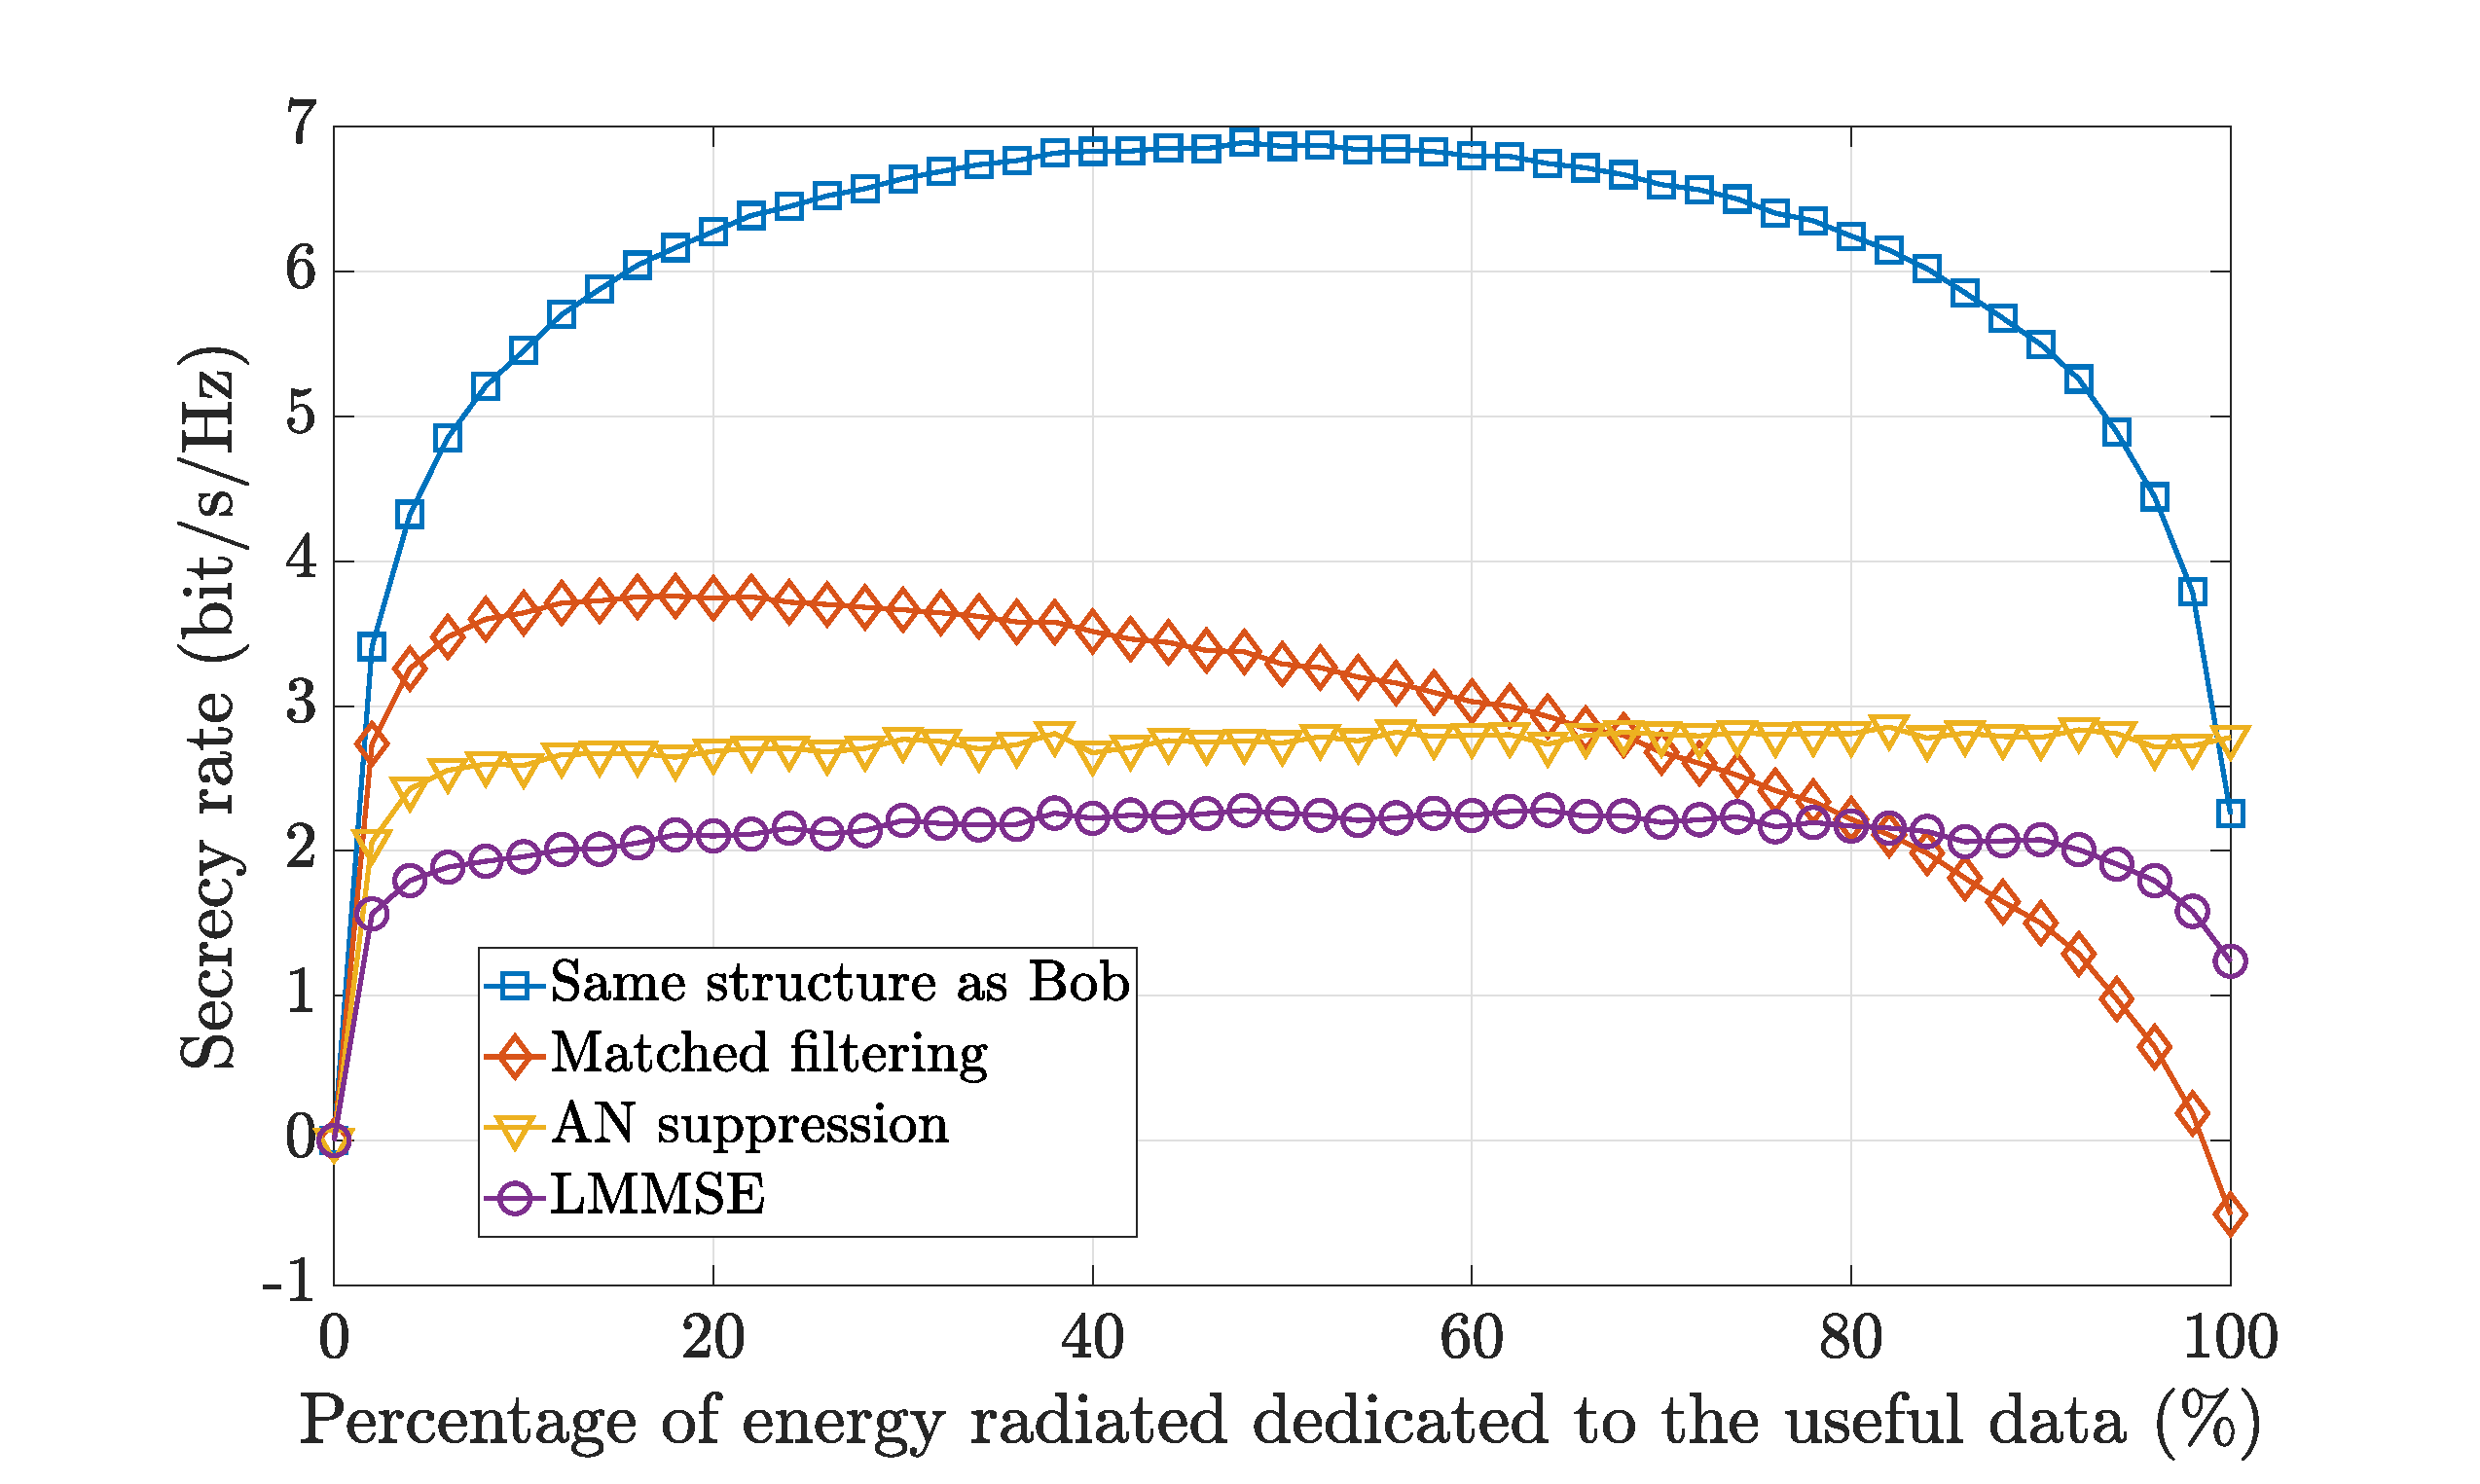
\includegraphics[width = .65\textwidth]{graphs/SR_filter_comparaison.eps}}
    \caption{Secrecy Rate curves for the different decoding structures at Eve, $E_b/N_0=20$ dB, BOR = 4 }
    \label{fig:secrecy_filt_comparaison}
\end{figure}
Fig.\ref{fig:secrecy_filt_comparaison} shows the secrecy performances for the 4 different structures implemented at the eavesdropper position, each of them assuming more computational resources and/or more knowledges at Eve as compared to Bob. It can be seen that when Eve implements the same receiving structure as Bob, the \gls{sr} is very high compared to the other curves, as anticipated from Section \ref{par:eve_same_bob}. When the \gls{an} killer algorithm is implemented, we observe that the curve remains flat, except for the situation where all the radiated energy is dedicated for the \gls{an} signal. The reason is that Eve's noise is amplify whatever the value of $\alpha$ since the \gls{an} signal is suppressed. The \gls{lmmse} curves exhibit the lower \gls{sr} sice it performs a decoding tradeoff between suppressing the \gls{an} and amplifying its noise, except for very high percentages of energy dedicated to the useful signal. Finally, we note that the \gls{sr} when Eve implements a matched filter is relatively low. Furthermore, it becomes negative when the transmitted signal only contains data. In fact, if Eve and Bob noise levels are identical, which is assumed throughout this report , the \gls{sinr} ratio when no \gls{an} is radiated becomes:
\begin{equation}
    \kappa \approx \frac{\EX{\gamma_{B,n}}}{\EX{\gamma_{E,n}}}\Big|_{\alpha \to 1} \approx \frac{\frac{U+1}{U}}{\left(\frac{U+1}{U}\right)^2} = \frac{U}{U+1}< 1
\end{equation}
giving rise to a negative \gls{sr}. The reason why the \gls{lmmse} decoding structure does not exhibit better decoding performances at Eve, i.e., lower \gls{sr} values, compared to the matched filter receiver for all values of $\alpha$ has not been explained yet.






\subsubsection{Waterfilling Optimization}
\label{subsub:simu_waterfilling}
\begin{figure}[htb!]
    \centering
    \centerline{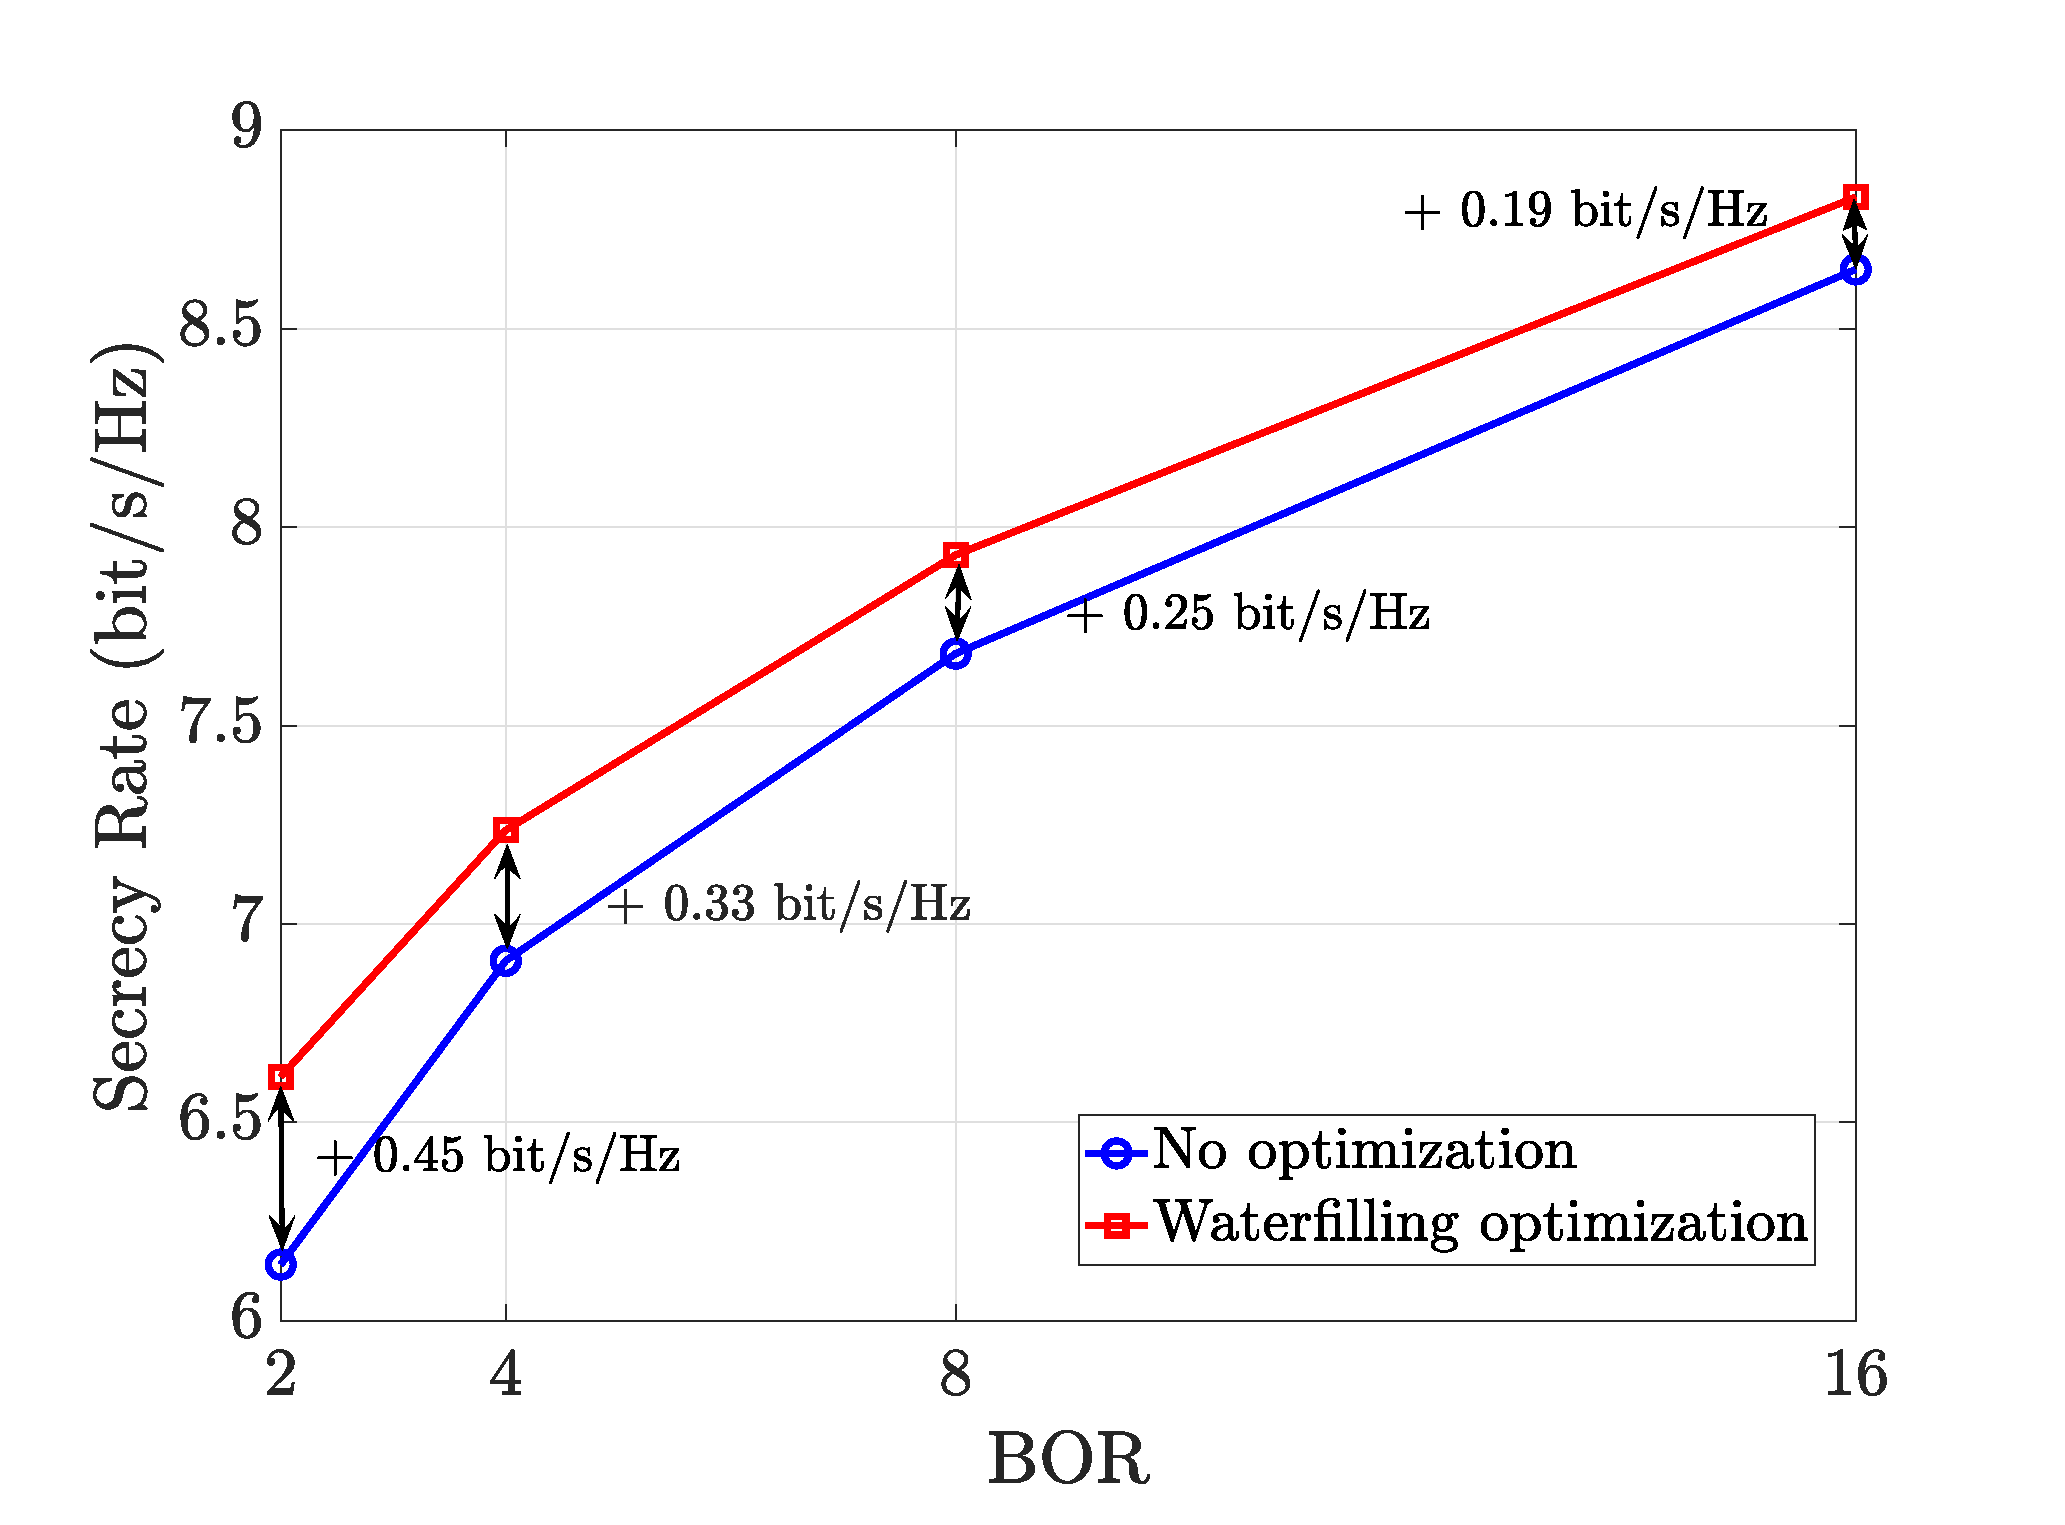
\includegraphics[width = .65\textwidth]{graphs/alpha_waterfilling.eps}}
    \caption{SR optimization via waterfilling, Bob and Eve with same capabilities, $E_b/N_0=20$ dB}
    \label{fig:waterfilling_opt_alpha}
\end{figure} 
Fig. \ref{fig:waterfilling_opt_alpha} presents the maximal values of the \gls{sr} obtained when Eve implements the despreading only receiving structure, i.e. the same structure as Bob, before and after waterfilling optimization. As a reminder, before and after optimization, the mean energy radiated dedicated to the useful data remains unchanged. This amount of energy is computed thanks to (\ref{eq:best_alpha}) in order to ensure a maximal \gls{sr}. This \gls{sr} is then further increased via the waterfilling optimization procedure, as described in section \ref{subsec:perf_waterf}. As we can see, there is an increase of the \gls{sr} for all \gls{bor} values thanks to the optimization. However, this increase decreases with an increase of the \gls{bor}. This can be explained since, when the \gls{bor} increases, the channel frequency diversity is better exploited by the \gls{tr} scheme. Therefore, it becomes more difficult to gain from the coefficient optimization procedure and the \gls{sr} is then less enhanced. 